\documentclass[tikz]{standalone}

\usepackage[latin1]{inputenc}
\usepackage{tikz}

% GNUPL
\usetikzlibrary{arrows}
\tikzset{
  arrow/.pic={\path[tips,every arrow/.try,->,>=stealth'] (0.08,0) -- +(.1pt,0);},
  rearrow/.pic={\path[tips,every arrow/.try,<-,>=stealth'] (-0.15,0) -- +(.1pt,0);},
}
\begin{document}
\pagestyle{empty}

\pgfmathsetmacro{\goldenRatio}{(1+sqrt(5)) / 2}

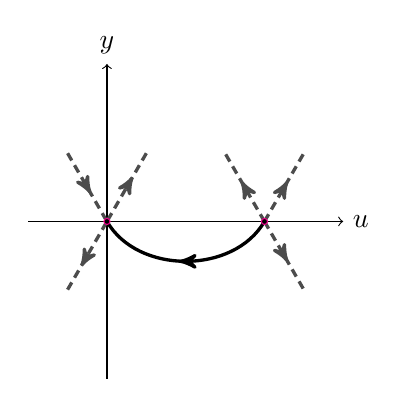
\begin{tikzpicture}[
    save/.style={opacity=0.3},
    xi/.style={thick,black, very thick},
    infty/.style={xi, black!70, densely dashed},
    harmonic/.style={thick, blue, save},
    orbita/.style={thick, black, save},
    saddle/.style={thick, black, save},
    outer/.style={thick, purple, save},
    nodes={sloped,allow upside down}
]
    %\draw[very thin,color=gray] (-1,1.1) grid (3.9,3.9);
    % \draw (0,0) rectangle (1,1);
    \draw[->]  (-1,0) -- (3,0) node[right] {$u$};
    \draw[->]  (0,-2) -- (0,2) node[above] {$y$};
	%фокус(-покус)

    % \draw[orbita] (0,0) to [out=80,in=180] (2,1);
    % \draw[orbita] (2,1) to [out=0,in=90] (3,0);
    % \draw[orbita] (0,0) to [out=-80,in=180] (2,-1);
    % \draw[orbita] (2,-1) to [out=0,in=-90] (3,0);
    % \draw[orbita] [->] (2,1) --(2.01,1);
    % \draw[orbita] [<-] (2,-1) --(2.01,-1);    

    % \draw[harmonic] (0.5,0) to [out=80,in=180] (2,0.8);
    % \draw[harmonic] (2,0.8) to [out=0,in=90] (2.78,0);
    % \draw[harmonic] (0.5,0) to [out=-80,in=180] (2,-0.8);
    % \draw[harmonic] (2,-0.8) to [out=0,in=-90] (2.78,0);
    % \draw[harmonic] [->] (2,0.8) --(2.01,0.8);
    % \draw[harmonic] [<-] (2,-0.8) --(2.01,-0.8);

    % \draw[harmonic] (1,0) to [out=80,in=180] (2,0.5);
    % \draw[harmonic] (2,0.5) to [out=0,in=90] (2.6,0);
    % \draw[harmonic] (1,0) to [out=-80,in=180] (2,-0.5);
    % \draw[harmonic] (2,-0.5) to [out=0,in=-90] (2.6,0);
    % \draw[harmonic] [->] (2,0.5) --(2.01,0.5);
    % \draw[harmonic] [<-] (2,-0.5) --(2.01,-0.5);


    % \draw[harmonic] (1.5,0) to [out=80,in=180] (2,0.3);
    % \draw[harmonic] (2,0.3) to [out=0,in=90] (2.3,0);
    % \draw[harmonic] (1.5,0) to [out=-80,in=180] (2,-0.3);
    % \draw[harmonic] (2,-0.3) to [out=0,in=-90] (2.3,0);
    % \draw[harmonic] [->] (2,0.3) --(2.01,0.3);
    % \draw[harmonic] [<-] (2,-0.3) --(2.01,-0.3);



	%седло
	\draw[infty] (120:1) -- pic{arrow} (0,0);	
    \draw[infty] (60:1) -- pic{rearrow} (0,0);
    \draw[infty] (-120:1) -- pic{rearrow} (0,0);
    % \draw[xi,densely dashed] (0.4,1.2) -- pic{rearrow} (0,0);

	% \draw[outer] (-0.4,0.8) to [out=-80,in=90] (-0.28,0);
	% \draw[outer] (-0.4,-0.8) to [out=80,in=-90] (-0.28,0);
	% \draw[outer] [->]  (-0.4,0.8) -- (-0.3,0.33);

	%не имеющие физ смысла
	% \draw[outer] (-0.4,1.5) to [out=-80,in=180] (0,1);
	% \draw[outer] (0,1) to [out=0,in=-180] (2,1.3);
	% \draw[outer] (2,1.3) to [out=0,in=90] (3.4,0);
	% \draw[outer] (-0.4,-1.5) to [out=80,in=180] (0,-1);
	% \draw[outer] (0,-1) to [out=0,in=-180] (2,-1.3);
	% \draw[outer] (2,-1.3) to [out=0,in=-90] (3.4,0);
	% \draw[outer] [->] (2,1.3) --(2.01,1.3);
	% \draw[outer] [<-] (2,-1.3) --(2.01,-1.3);


    % \draw[xi,densely dashed]  (0,0) .. controls (0.5,1.85) and (3.7,2) ..  pic{arrow}  (4,0);

 % \pgfmathsetmacro{\offset}{rad(atan(2*ln(\goldenRatio)/pi))};
 %  \draw[xi, xshift=2cm,domain=0:2.88*pi,
 %       samples=600,variable=\t] plot
 %   ({\t/20*sin(\t r)},
 %    {\t/20*cos(\t r)}) 
 %   coordinate(end);

   \draw[xi] (2,0) to [out=-120,in=-60] pic{arrow} (0,0);
    \draw[infty] (2,0) -- pic{arrow} ++(60:1);    
    \draw[infty] (2,0) -- pic{arrow} ++(120:1);    
    \draw[infty] (2,0) -- pic{arrow} ++(-60:1);    

   \draw[magenta, fill=black] (0,0) circle (1.1pt);
   \draw[magenta, fill=black] (2,0) circle (1.1pt);



    % %поток траекторий
    % \draw[gray, thick, ] [->] (2,0.4) --(2.3,0.6);
    % \draw[gray, thick, ] [->] (2.4,0.3) --(2.7,0.5);
    % \draw[gray, thick, ] [->] (1.7,0.8) --(2.1,1.1);
    % \draw[gray, thick, ] [->] (2.1,0.1) --(2.35,0.3);
    % \draw[gray, thick, ] [->] (2.1,-0.8) --(1.8,-1.1);
    % \draw[gray, thick, ] [->] (1.8,-0.4) --(1.5,-0.7);
    % \draw[gray, thick, ] [->] (1.4,-0.8) --(1.1,-1);

    % %ветви
    % \draw[red, thick, ] (-0.5,1) to [out=-50,in=110] (-0.25,0.5);
    % \draw[red, thick, ] (-0.25,0.5) to [out=-70,in=120] (0,0);
    % \draw[red, thick, ] (0,0) to [out=-60,in=180] (1.3,-0.5);
    % \draw[red, thick, ] (1.3,-0.5) to [out=0,in=-90] (2.2,0);
    % \draw[red, thick, ] (2.2,0) to [out=90,in=0] (2,0.17);
    % \draw[red, thick, ] (2,0.17) to [out=180,in=90] (1.83,0);
    % \draw[thick, ] [red, ->] (-0.25,0.51) --(-0.24,0.49);
    % \draw[thick, ] [red, ->] (0.25,-0.255) --(0.24,-0.245);

    % \draw[cyan, thick, ] (-0.25,-1) to [out=70,in=-100] (-0,0);
    % \draw[cyan, thick, ] (-0,0) to [out=80,in=-180] (2,1.8);
    % \draw[cyan, thick, ] (2,1.8) to [out=0,in=90] (4.2,0);
    % \draw[thick, ] [cyan, ->] (0.2,0.63) --(0.25,0.75);
    % \draw[thick, ] [cyan, ->] (0,0) --(-0.16,-0.75);

    % % \coordinate [label=center:$1$] (1) at (1,0);
    % \draw[red] (-0.5,1) node[left] {$stable$};
    % \draw[cyan] (5.8,0.3) node[left] {$unstable$};
    % \coordinate [label=right:$\nu \ll 1$] (nu) at (3,2);
    % \draw [fill] (2,0) circle [radius=0.01];
    % \draw [fill] (2.6,0) circle [radius=0.03];
    % \draw [fill] (3,0) circle [radius=0.03];
\end{tikzpicture}


\end{document}